
%\documentclass{elsart}               % The use of LaTeX2e is preferred.

\documentclass[twocolumn]{autart}    % Enable this line and disable the 
                                     % preceding line to obtain a two-column 
                                     % document whose style resembles the
                                     % printed Automatica style.


\usepackage{graphicx}          % Include this line if your 
                               % document contains figures,
%\usepackage[dvips]{epsfig}    % or this line, depending on which
                               % you prefer.

\usepackage{graphicx}
\usepackage[utf8]{inputenc}

%\usepackage[spanish]{babel}
\usepackage{geometry}


\usepackage{ntheorem,lipsum}

\theorembodyfont{\upshape}
\newtheorem{thm}{Teorema}[section]
\newtheorem{definition}{Definition}[section]
\newtheorem{obs}{Observación}[section]
\newtheorem{proposition}{Proposition}[section]
\newtheorem{example}{Ejemplo}[section]
\newtheorem{problem}{Problem}[section]
\newtheorem{hipo}{Hipotesís}[section]

\usepackage{bm}

\usepackage{amsmath}
\usepackage{amssymb}

\DeclareMathOperator*{\argmax}{arg\,max}
\DeclareMathOperator*{\argmin}{arg\,min}
\usepackage{hyperref}
\hypersetup{
    colorlinks=true,
    linkcolor=blue,
    filecolor=magenta,      
    urlcolor=cyan,
}


\numberwithin{equation}{section}


\usepackage[Algoritmo]{algorithm}

\usepackage{algpseudocode}
\usepackage{caption}
\usepackage{subcaption}

\begin{document}

\begin{frontmatter}
\runtitle{Selective Harmonic Elimination via Optimal Control}   % Running title for regular 
                                              % papers but only if the title  
                                              % is over 5 words. Running title 
                                              % is not shown in output.

\title{Piece-wise penalization in Optimal Control to Selective Harmonic Elimination} % Title, preferably not more 
                                                 % than 10 words.

\thanks[footnoteinfo]{This paper was not presented at any IFAC 
meeting.}

\author[FD,UD]{Umberto Biccari}\ead{umberto.biccari@deusto.es},    % Add the 
\author[UAM,FD]{Carlos Esteve}\ead{carlos.esteve@uam.es},               % e-mail address 
\author[UD]{Jes\'us Oroya}\ead{djoroya@deusto.es}  % (ead) as shown
\address[FD]{Chair of Computational Mathematics, Fundaci\'on Deusto, Avenida de las Universidades 24, 48007 Bilbao, Basque Country, Spain.}  %
\address[UD]{Universidad de Deusto, Avenida de las Universidades 24, 48007 Bilbao, Basque Country, Spain.}  %
\address[UAM]{Departamento de Matem\'aticas, Universidad Aut\'onoma de Madrid, 28049 Madrid, Spain.}  % Please supply                                              
          
\begin{keyword}                           % Five to ten keywords,  
Selective Harmonic Elimination; Finite Set Control, Piecewise Linear function.               % chosen from the IFAC 
\end{keyword}                             % keyword list or with the 
                                          % help of the Automatica 
                                          % keyword wizard


\begin{abstract}                          % Abstract of not more than 200 words.
El problema de \emph{Selective Harmonic Elimination pulse-width modulation}(SHE) es planteado como el problema de control óptimo, con el fin de encontrar soluciones de ondas escalón sin prefijar el número de ángulos de conmutación. De esta manera, la metodología de control óptimo es capaz de encontar la forma de onda óptima y de encontrar la localizaciones de los ángulos de conmutación, incluso sin prefijar el número de conmutaciones. Este es un nuevo enfoque para el problema SHE en concreto y para los sistemas de control con un conjunto finito de controles admisibles en general.

\end{abstract}

\end{frontmatter}


\section{Introduction and motivations}\label{Section1}

Selective Harmonic Elimination (SHE) \cite{Rodriguez2002} is a well-known methodology in electrical engineering, employed to improve the performances of a converter by controlling the phase and amplitude of the harmonics in its output voltage. As a matter of fact, this technique allows to increase the power of the converter and, at the same time, to reduce its losses. 

In broad terms, the process consists in generating a \textit{control signal} with a desired harmonic spectrum, by modulating or eliminating some specific lower order frequencies. This signal is in the shape of a step function and is fully characterized by two features (see Figure \ref{fig:exampleSHE}): 
\begin{itemize}
	\item[1.] The \textit{waveform}, i.e. the set of (constant) values the function may assume.
	\item[2.] The \textit{switching angles}, defining the points in the domain where the function changes from one constant value to another. 
\end{itemize}



Because of the growing complexity of modern electrical networks, consequence for instance of the high penetration of renewable energy sources, the demand in power of electronic converters is day by day increasing. For this and other reasons, SHE has been a preeminent research interest in the electrical engineering community, and a plethora of SHE-based techniques has been developed in recent years. An incomplete bibliography includes \cite{duranay2017selective,Janabi2020,Yang2017}.

Nowadays, SHE is mostly based on offline computations to obtain the commutation patterns describing the control signal.  

\textcolor{red}{Add references and mention real-time approaches.}

\textcolor{red}{Estructura del documento}

%The present document is organized as follows. In Section \ref{Section2}, we will present the mathematical formulation of the SHE problem and a classical resolution method based on an optimization process. In Section \ref{Section3}, we will formulate the SHE problem as a controlled dynamical system. In Section \ref{Section4}, we will present the optimal control problem allowing us to obtain the solutions to the SHE problem. In Section \ref{Section5}, we will present our numerical experiments. Finally, in Section \ref{Section6}, we will equation the conclusions of our study.


\section{Mathematical formulation of SHE}\label{Section2}

This section is devoted to the mathematical formulation of the SHE problem. In what follows, with the notation $\mathcal U$ we will always refer to a finite set of real numbers, contained in the interval $[-1,1]$
\begin{align}\label{eq:Udef}
	\mathcal U = \{u_\ell\}_{\ell=1}^L\subset [-1,1],
\end{align}
with cardinality $|\mathcal U| = L$. 

In broad terms, our objective is to design a piece-wise constant function $u(\tau):[0,2\pi)\to\mathcal U$ such that some of its lower-order Fourier coefficients take specific values determined a priori. 

 
\begin{figure}
	\centering
	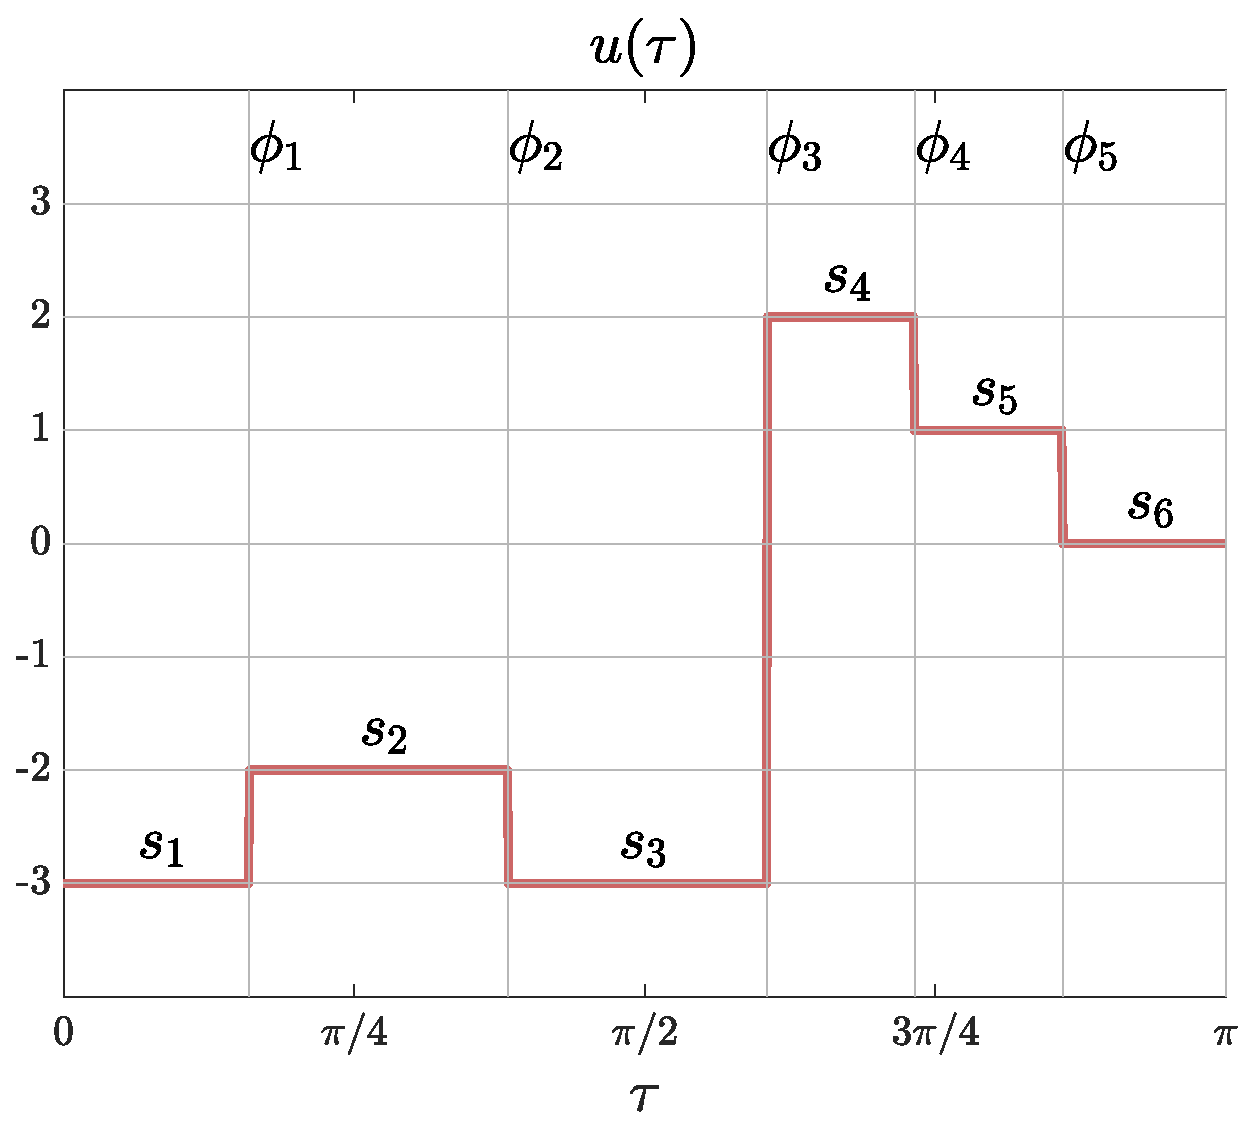
\includegraphics[scale=0.35]{img/fig01.eps} 
	\caption{A Step function and possible solution of Problem \ref{pb:SHEp}, where we considered a possible finite set of control $\mathcal{U} = \{-1/3, -2/3, 0, 1/3, 2/3, 1\}$. We show the switching angles $\bm{\phi}$ and the waveform $\mathcal{S}$ (see Definitions \ref{def:waveform} and \ref{def:switchingAngles}). \textcolor{red}{tengo que darle la vuelta en el tiempo}}\label{fig:exampleSHE}
\end{figure}

Due to the application in power converters, we will focus here on functions with \textit{half-wave symmetry}, i.e. 
\begin{align*}
	u(\tau + \pi) = -u(\tau)\quad \mbox{for all}\; \tau \in [0,\pi).
\end{align*}
In this way, $u$ is fully determined by its values in the interval $[0,\pi)$ and its Fourier series only involves the odd terms, thus taking the form
\begin{equation}
	u(\tau ) = \sum_{\underset{i\, odd}{i \in \mathbb{N}}} a_i \cos(i\tau)+ \sum_{\underset{j\, odd}{j \in \mathbb{N}}}  b_j \sin(j \tau), 
\end{equation}
where the coefficients $a_i$ and $b_j$ are given by
\begin{equation} \label{eq:an}
	\begin{aligned}
		a_i = \frac{2}{\pi} \int_0^\pi u(\tau ) \cos(i \tau)\,d\tau, 
		\\
		b_j = \frac{2}{\pi} \int_0^\pi u(\tau)  \sin(j \tau)\,d\tau.
	\end{aligned}
\end{equation}
Because of this half-wave symmetry, in what follows, we will always work with the restriction $u|_{[0,\pi)}$ which, with some abuse of notation, we shall still denote by $u$. We can then give a general formulation of the SHE problem as follows:
\newline
\begin{problem}[SHE]\label{pb:SHEp}
Let $\mathcal{E} _a $ and $\mathcal{E} _b $ be two sets of odd numbers with cardinalities $|\mathcal{E}_a| = N_a $ and $ |\mathcal{E} _b| = N_b$, respectively, and $\mathcal{U}$ be defined as in \eqref{eq:Udef}. Given the vectors $\bm{a}_T \in \mathbb{R}^{N_a}$ and $\bm{b}_T \in \mathbb{R}^{N_b} $, we look for a piece-wise constant function $u: [0,\pi)\to\mathcal{U}$ such that 
\begin{gather}
	\notag a_i = (\bm{a}_T)_i, \quad\textrm{ for all } i \in \mathcal{E}_a,
	\\
	\notag b_j = (\bm {b}_T)_j, \quad\textrm{ for all } j \in \mathcal{E}_b,
\end{gather}
with $\{a_i\}_{i\in\mathcal E_a}$ and $\{b_j\}_{j\in\mathcal E_b}$ given by \eqref{eq:an}.
\end{problem} 
 
Fig. \ref{fig:exampleSHE} shows an example of a function $u$ solution of the SHE problem. 



\section{Classical approach to the SHE problem}

En esta sección presentaremos la aproximación actual que se utiliza para abordar el problema, y mencionaremos sus problemas asociado. As we anticipated in Section \ref{Section1}, the control signal $u$ is fully characterized by its waveform and the switching angles, to which we now give a precise definition.
\newline
\begin{definition}[Wave-form]\label{def:waveform}
Given the finite set $\mathcal U$ defined in \eqref{eq:Udef} and $M\in\mathbb{N}$, we will call a waveform any possible $(M+1)$-tuple $\mathcal S = (s_m)_{m=1}^{M+1}$ with $s_m\in \mathcal U$ for all $m=1,\ldots,M+1$.
\end{definition}
\vspace{1em}
\begin{definition}[Switching angles]\label{def:switchingAngles}
Given the finite set $\mathcal U$ defined in \eqref{eq:Udef}, $M\in\mathbb{N}$ and a piece-wise constant function $u:[0,\pi) \rightarrow \mathcal{U}$, we shall refer as switching angles $\bm{\phi} = \{\phi_m\}_{m=0}^{M+1}\subset[0,\pi]$, with $\phi_0 = 0$ and $\phi_{M+1} = \pi$, to the points in the domain $[0,\pi)$ where $u$ changes its value. 
\end{definition}

In view of the above definitions, we can provide the following explicit expression for $u$:
\begin{align}\label{eq:uExpl}
	&u = \sum_{m=1}^{M+1} s_m\chi_{[\phi_m,\phi_{m+1}]}
	\\
	&s_m\in\mathcal S, \;\phi_m\in{\bm{\phi}}, \quad \mbox{for all } m=1,\ldots,M+1, \notag 
\end{align}
where we denoted by $\chi_{[\phi_m,\phi_{m+1}]}$ the characteristic function of the interval $[\phi_m,\phi_{m+1}]$.

Besides, taking into account \eqref{eq:uExpl}, a direct computation yields that the Fourier coefficients \eqref{eq:an} are given by
\begin{align*}
	& a_i = a_i(\bm{\phi}) =  \frac{2}{i\pi} \sum_{k=1}^{M+1} s_k \Big[\sin(i\phi_k) -\sin(i\phi_{k-1})\Big]
	\\
	& b_j = b_j(\bm{\phi}) = \frac{2}{j\pi} \sum_{k=1}^{M+1} s_k \Big[\cos(j\phi_{k-1}) -\cos(j\phi_{k})\Big]
\end{align*}
Given a waveform $\mathcal S$, Problem \ref{pb:SHEp} then reduces to find the switching locations $\bm{\phi}$ (see \cite{Yang2015,Konstantinou2010,Sun1996}). This can be cast as a minimization problem in the variables $\{\phi_m\}_{m=0}^{M+1}$, where the cost functional is the Euclidean distance between the obtained Fourier coefficients $\{a_i(\bm{\phi}),b_j(\bm{\phi})\}$ and the targets $(\bm{a},\bm{b})\in \mathbb{R}^{N_a}\times \mathbb{R}^{N_b}$.
\newline
\begin{problem}[Optimization for SHE]
Given a waveform $\mathcal S$ and a step function $u$ in the form \eqref{eq:uExpl}, we look for the switching angles locations $\bm{\phi}$ by means of the following minimization problem:
\begin{align}
	&\min_{\bm{\phi} \in [0,\pi]^{M}} \left(\sum_{i\in\mathcal{E}_a} \|a_T^i - a_i(\bm{\phi})\|^2 + \sum_{j\in \mathcal{E}_b} \|b_T^j - b_j(\bm{\phi})\|^2\right)\notag 
	\\[10pt]
	&\mbox{subject to: } 0 = \phi_0 <\phi_1 < \ldots < \phi_{M} < \phi_{M+1} = \pi \notag 
\end{align}
\end{problem}
A continuación mecionaremos algunos problemas de esta formulación:
\begin{enumerate}
    \item \textbf{Combinatory problem}: Since the cardinality of $\mathcal S$ is not known a priori, meaning that we do not know how many switches will be necessary to reach the desired values of the Fourier coefficients, a common approach to solve the SHE problem consists in fixing the number of changes and generating all the possible combinations of elements of $\mathcal S$, to later solve an optimization problem for each one of them. Nevertheless, taking into account that the number of possible tuples $\mathcal S$ is given by $|\mathcal{U}|^{|\mathcal S|}$, it is evident that the complexity of the above approach increases rapidly. This problem has been studied in \cite{Yang2015} where, through appropriate algebraic transformations, the authors are able to convert the SHE problem into a polynomial system whose solutions' set contains all the possible waveforms for a given set $\mathcal{U}$ and number of elements in the sequence $\mathcal S$.  Sin embargo, en este caso el número de cambios es prefijado.
	%\item \textbf{Real-time problem}: We shall also mention that the SHE methodology has been developed to provide in real-time different target Fourier coefficients con with a $KHz$ latency. This makes impossible to find real-time solutions by optimization, making then necessary to pre-determine solutions that can later be interpolated. 
	\item \textbf{Continuity problem}: It is well-known that, fixed a sequence $S$, the continuity of the switching locations with respect to a continuous variation of the target Fourier coefficients may be quite cumbersome. De manera que, encontrar solución donde el número de ángulos pueda cambiar con el vector objetivo, nos puede dar más libertad para obtener soluciones más predecibles. 
\end{enumerate}
%
%

%
%

\section{Our Contributions}

We will present the SHE problem as an optimal control one, where the optimization variable is the signal $u(\tau)$ defined in the entire interval $[0,\pi)$. 
%
In particular, we will describe how the Fourier coefficients of the function $u(\tau)$ can be seen as the final state of a system controlled by $u (\tau)$. Hence, the optimization is performed among all the possible functions that satisfy $|u(\tau)|<1 $ and can control the final state at the desired Fourier coefficients. Then we will show how to design a control problem so that the solution is a step function.
 
In this way, we can reformulate Problem \ref{pb:SHEp} as follows.
\newline
In this formulation, the SHE problem converts in a minimization problem with restrictions which can be solved by well-known techniques. Since the problem has several minimizers, we shall solve it employing global optimizers. Furthermore, since the choice of the waveform is arbitrary, we shall proceed in the same way for each possible waveform. 

\subsection{Reformulation of SHE problem as optimal control problem}

%As we anticipated in Section \ref{Section1}, the main contribution of the present paper is to provide a novel and alternative approach to the SHE problem, based on optimal control. As we shall see, this methodology will allow us avoiding the choice of the waveform, as the optimization process selects the most convenient one in each case. 
%\newline

Teniendo en cuenta tenemos todos los elementos considerados en la definición del Problema \ref{pb:SHEp}, introducimos el siguiente sistema dinámico:

\begin{equation}\label{eq:CauchyReversed}
    \begin{cases}
        \displaystyle\dot{\bm{x}}(\tau) = -\frac 2\pi\bm{\mathcal{D}}(\tau)u(\tau),  & \tau \in [0,\pi)
        \\[6pt]
        \bm{x}(0) = \bm{x}_0
    \end{cases},
\end{equation}
Where $\bm{x}(t) \in \mathbb{R}^{N_a + N_b}$ and $\bm{\mathcal{D}}(\tau) \in  \mathbb{R}^{N_a + N_b}$ are:
\begin{align*}
	\bm{x}(\tau) = \begin{bmatrix} \bm{\alpha}(\tau) \\ \bm{\beta}(\tau) \end{bmatrix}, \quad
	\bm{\mathcal{D}}(\tau) = \begin{bmatrix} \bm{\mathcal{D}}^\alpha(\tau) \\ \bm{\mathcal{D}}^\beta(\tau) \end{bmatrix}     
\end{align*}
y donde:
\begin{align*}
	\bm{\mathcal{D}}^\alpha(\tau) = 
	\begin{bmatrix} 
		\cos(e_a^1\tau) \\ \cos(e_a^2\tau) \\ \vdots \\ \cos(e_a^{N_a}\tau) 
	\end{bmatrix},
	\quad \bm{\mathcal{D}}^\beta(\tau) = 
	\begin{bmatrix} 
		\sin(e_b^1\tau) \\ \sin(e_b^2\tau) \\ \vdots \\ \sin(e_b^{N_b}\tau) 
	\end{bmatrix} 
\end{align*}
with $\bm{\mathcal{D}}^\beta(\tau) \in \mathbb{R}^{N_a} $ and $ \bm{\mathcal{D}}^\beta(\tau) \in \mathbb{R}^{N_b}$, and where the set $\mathcal{E}_a$ and $\mathcal{E}_b$ are:
\begin{align*}
	\mathcal{E}_a = \{e_a^1,e_a^2,e_a^3,\dots,e_a^{N_a}\}, \quad \mathcal{E}_b = \{e_b^1,e_b^2,e_b^3,\dots,e_b^{N_b}\}    
\end{align*}
%
Además proponemos el siguiente problem de control:
\vspace{1em}
\begin{problem}\label{pb:SHEpControl}
    Let $\mathcal{U}$ be defined as in \eqref{eq:Udef} and let $\mathcal{E} _a $ and $\mathcal{E} _b $ be two sets of odd numbers with cardinalities $|\mathcal{E}_a| = N_a $ and $ |\mathcal{E} _b| = N_b$, respectively. Given the vectors $\bm{a}_T \in \mathbb{R}^{N_a}$ and $\bm{b}_T \in \mathbb{R}^{N_b} $, let us define $\bm{x}_0=[\bm{a}_T,\bm{b}_T]^\top \in \mathbb{R}^{N_a}\times\mathbb{R}^{N_b}$. We look for $u:\in [0,\pi)\to\mathcal{U}$ such that the solution of \eqref{eq:CauchyReversed} with initial datum $\bm{x}(0)=\bm{x}_0$ satisfies $\bm{x}(\pi)=0$.
\end{problem}
\vspace{1em}

\begin{theorem}
    El control óptimo $u(\tau)$, solución del Problema \ref{pb:SHEpControl}, es el función constante a trozos que resuleve el Problema \ref{pb:SHEp}.   
\end{theorem}

\begin{figure}[ht!] 
    \centering
    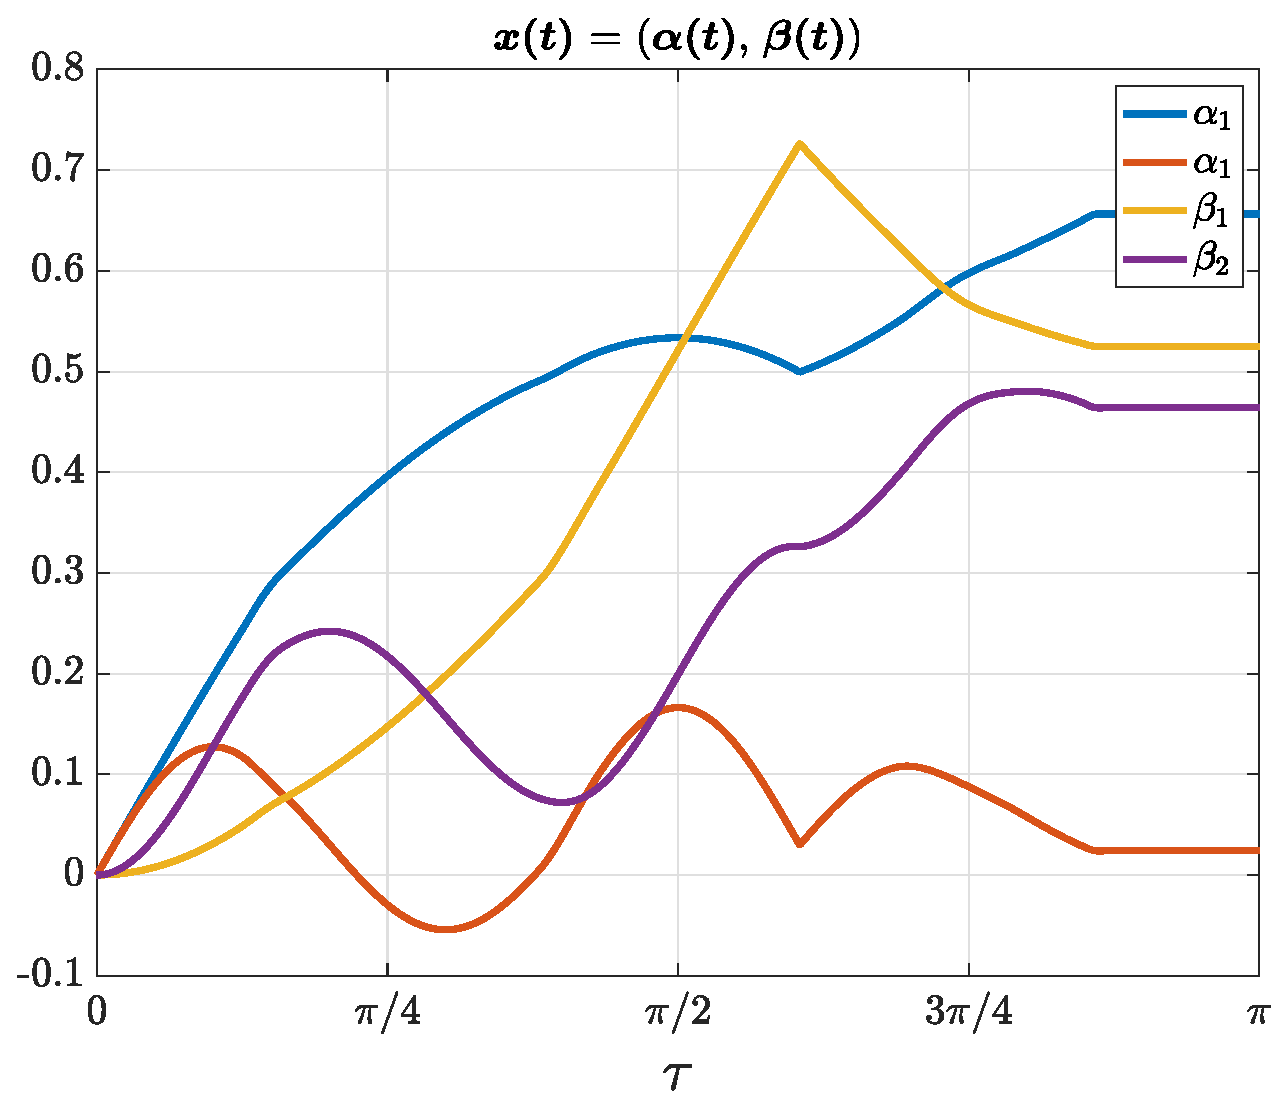
\includegraphics[scale=0.35]{img/fig02.eps}
    \caption{Evolución del sistema dinámico con los conjuntos $\mathcal{E}_a = \{1,2\}$ y $\mathcal{E}_b = \{1,2\}$ considerando el control $u(\tau)$ presentado en la Figura \ref{fig:exampleSHE}. Además mostramos las posiciones de los ángulos de conmutación $\bm{\phi}$.}
\end{figure}

\vspace{1em}
\begin{remark}[Quarter-wave symmetry]
    We shall mention that, in the SHE literature, it is usual to distinguish among the half-wave symmetry problem (addressed in the present paper) and the quarter-wave symmetry one in which
    \begin{align*}
        u\left(\tau + \frac \pi2\right) = -u(\tau)\quad \mbox{for all}\; \tau \in \left[0,\frac \pi2\right).
    \end{align*}
    In quarter-wave symmetry, the SHE problem simplifies, as the Fourier coefficients $\{a_i\}_{i\in\mathcal E_a}$ turn out to be all zero. Hence, only the phases of the converter's signal can be controlled, while the half-wave SHE allows to deal with the amplitudes as well. It is worth to remark nonetheless that our optimal control formulation can be easily adapted to the quarter-wave symmetry problem by simply replacing the Fourier coefficients \eqref{eq:an} with
    \begin{align*}
        a_i = 0, \quad\quad b_j = \frac{4}{\pi} \int_0^{\frac \pi4} u(\tau)  \sin(j \tau)\,d\tau.
    \end{align*}
    Entonces podemos introducir el siguiente sistema dinámico:
    \begin{gather}
        \begin{cases}
            \displaystyle \dot{\bm{\beta}}(\tau) = \frac 2\pi \bm{\mathcal{D}}^\beta(\tau) u(\tau), & \tau \in [0,\pi/2)
            \\[6pt]
            \bm{\beta}(0) = \bm{b}_T
        \end{cases}\label{eq:CauchyReversed_4sym}
    \end{gather}
    Además del siguiente problema de control:
    \vspace{0.5em}
    \begin{problem}\label{pb:SHEpControl_4sym}
        Let $\mathcal{U}$ be defined as in \eqref{eq:Udef} and let $\mathcal{E} _b $ be a set of odd numbers with cardinality $ |\mathcal{E} _b| = N_b$. Given the vector $\bm{b}_T \in \mathbb{R}^{N_b} $. We look for $u:\in [0,\pi/2)\to\mathcal{U}$ such that the solution of \eqref{eq:CauchyReversed_4sym} with initial datum $\bm{x}(0)=\bm{x}_0$ satisfies $\bm{x}(\pi)=0$.
    \end{problem}
    Donde de la misma forma que en el problema con simetría de media onda la solución de este problema es también solución del problema SHE con simetría de cuarto de onda.
\end{remark}


%As we anticipated in Section \ref{Section3}, the SHE problem is equivalent to controlling a dynamical system associated with the Fourier coefficients \eqref{eq:an}. In this section, we present a rigorous formulation of this mentioned control problem and we analyze some relevant properties. 

In what follows, for a given vector $\bm{v}\in\mathbb{R}^d$, we shall always denote by $\|\bm{v}\|$ the euclidean norm $\|\bm{v}\|_{\mathbb{R}^d}$.
\newline


\begin{problem}[OCP for SHE]\label{pb:OCP1}
Let $\mathcal U$ be defined as in \eqref{eq:Udef}. Given two sets of odd numbers $\mathcal {E}_a $ and $\mathcal {E}_b $ with cardinality $N_a$ and $N_b$, respectively, and given the target $\bm{x}_T\in \mathbb{R}^{N_a+N_b}$, we look for the function $u(\tau):[0,\pi)\to \mathcal U$ solution of the optimal control problem  
\begin{align*}
	&\min_{u \in \mathcal{U}}\;\frac 12 \|\bm{x}(\pi)\|^2
	\\
    &\notag \text{subject to: }\quad \begin{cases}
            \displaystyle \dot{\bm{x}}(\tau) = -\frac 2\pi\bm{\mathcal{D}}(\tau) u(\tau),  & \tau \in [0,\pi)\\[6pt]
            \bm{x}(0) = \bm{x}_0
    \end{cases}
    \end{align*}
\end{problem}
The solution of Problem \ref{pb:OCP1} may be quite complex to be obtained, due to the restriction on the admissible control values. 

In order to bypass this difficulty, following a standard optimal control approach, we can formulate an equivalent minimization problem in which, instead of looking for $u\in\mathcal U$, we simply require that $|u|<1$ and we introduce a penalization term to ensure that $u$ is a piece-wise constant function (\textcolor{red}{digital control}). 

\vspace{0.5em}
\begin{definition}[Digital control of set $\mathcal{U}$]
A control $u(\tau)$ is called digital if, for each time $\tau\geq 0$, it only takes values in the finite set of real number $\mathcal{U}$ except a finite set of values.  
\end{definition}
%
This alternative optimal control problem, which can be solved more easily by employing standard tools, reads as follows:
\newline
\begin{problem}[Penalized OCP for SHE]\label{pb:OCP2}
Fix $\epsilon>0$. Given two sets of odd numbers $\mathcal E_a $ and $\mathcal E_b $ and the target $\bm{x}_T \in \mathbb {R}^{N_a + N_b}$, we look for the  function $u:[0,\pi)\to\mathcal U$ as the solution of:
\begin{align*}
	&\min_{|u|<1} \Bigg[\frac 12 \|\bm{x}(\pi) \|^2+ \epsilon \int_0^{\pi} \mathcal{L}(u(\tau)) d\tau \Bigg]  
\end{align*}
under the dynamics given by \eqref{eq:CauchyReversed}.
\end{problem}

In Problem \ref{pb:OCP2}, the penalization function $\mathcal L: \mathbb{R} \rightarrow \mathbb{R}$ will be chosen such that the optimal control $u^*$ only takes values in $\mathcal U$. Furthermore, the parameter $\epsilon$ should be small so that the solution minimizes the distance from the final state and the target.

%Next we will study the optimality conditions of the problem, for a general $\mathcal L$, and then specify how $\mathcal L$ should be so that the optimal control $u^*$ only takes the allowed values in $\mathcal U$.


\subsection{SHE bi-nivel via OCP (Bang-Bang Control)}

\begin{theorem}\label{th:bang-bang}
    Dado el Problema \ref{pb:OCP2} con el conjunto admisible de control $ \ \mathcal{U} = \{-1,1\}$. Si la función $\mathcal{L}$ es concava en el intervalo $[-1,1]$ del Problema \ref{pb:OCP2}, entonces la solución de problema es un control digital del conjunto $\mathcal{U} =  \{-1,1\}$.
\end{theorem}


\subsection{SHE multi-nivel via Piecewise linear penalization}

\begin{theorem}
    Dado un conjunto $\mathcal{U}$, we can choose the affine interpolation of a parabola $\mathcal{L}:[-1,1] \rightarrow \mathbb{R}$ as a penalization term. That is
    \begin{gather}\label{PLP}
        \mathcal{L}(u) = \begin{cases}
            \big[ (u_{k+1}+u_{k}) (u-u_k) + u_k^2 \big] & \text{if }  u \in [u_k,u_{k+1}[ \\
            1 & \text{if } u = u_{N_u} 
        \end{cases} \\
        \notag \forall k \in \{1,\dots,N_u-1\}
    \end{gather}
    De modo que el problema de \ref{pb:OCP2} con la penalización $\mathcal{L}(u)$ presentada antes tiene como solución un control digital del conjunto $\mathcal{U}$
\end{theorem}
\subsection{General conditions for  SHE multi-nivel}   

\begin{theorem}
    Assume that the finite set $\mathcal{U}$ defined in \eqref{eq:Udef} is composed by elements in ascending order. Let $\mathcal{Y} = \{y_\ell\}_{\ell=1}^L$ be another finite set, with the same cardinality as $\mathcal U$, such that the $L-1$ tuple
    \begin{gather}
        \frac{\Delta \mathcal{Y}}{\Delta \mathcal{U}} = \Bigg( \frac{y_\ell - y_{\ell+1}}{u_\ell - u_{\ell+1}} \Bigg)_{\ell=1}^{L-1}
    \end{gather}  is monotone. Let $\mathcal{L}:\mathbb{R} \rightarrow \mathbb{R}$ be a piece-wise continuous function:
    \begin{gather}
        \mathcal{L}(u) = \begin{cases}
            \mathcal{L}_k(u) & \text{if }  u \in [u_k,u_{k+1}[ \\
            1 & \text{if } u = u_{N_u} 
        \end{cases} \\
        \notag \forall k \in \{1,\dots,N_u-1\}
    \end{gather}    
    tal que $\{y_l = \mathcal{L}(u_l)\}_{l=1}^L$. Si las funciones $\mathcal{L}_k$ para todo $k \in  \{1,\dots,N_u-1\}$  son funciones concavas, entonces la penalización $\mathcal{L}$ en el problema \ref{pb:OCP2} da lugar a un control digital de $\mathcal{U}$.
\end{theorem}
\section{Numerical simulations}\label{Section5}

In this section, we will present several examples in which we solve our optimal control problem through the direct method and the non-linear constrained optimization tool \texttt{CasADi} \cite{Andersson2019}.
%
\subsection{Smooth approximation of piece-wise linear penalization}

With the final aim of using an optimization software to solve our optimal control problem, we will approximate our piece-wise linear penalization with the help of the Heaviside function $h:\mathbb{R} \rightarrow \mathbb{R}$ and its smooth approximation defined as follows: 
\begin{gather}
    h(x) = \begin{cases}
        1 & \text{ if } x \geq 0 \\
        0 & \text{ if } x < 0
    \end{cases}    
    \hspace{2em} 
    \begin{cases}
        h^\eta(x) = (1 + \tanh(\eta x))/2   \\
        \eta \rightarrow \infty
    \end{cases}
\end{gather}
Using $h$, we can define the (smooth) function $\Pi_{a,b}^\eta:\mathbb{R} \rightarrow \mathbb{R}$ as:
\begin{align*}
    \Pi_{[a,b]}^\eta(x) &= - 1 + h^\eta(x-a) + h^\eta(-x+b) 
    \\
    &= \frac{\tanh[\eta( x -a)] + \tanh[\eta (b-x)]}{2}.
\end{align*}
In this way, we can define the smooth version of \eqref{PLP}:
\begin{gather}
    \mathcal{L}^\eta(u) = \sum_{k = 1}^{N_u-1} \big[ (u_{k+1}+u_{k}) (u-u_k) + u_k^2 \big] \Pi^\eta_{[u_k,u_{k+1}]}(u)
\end{gather}
So that, when $\eta \rightarrow \infty$, then $\mathcal{L}^\eta \rightarrow \mathcal{L}$.

\subsection{Direct method  for  OCP-SHE}

To solve the optimal control problem (\ref{pb:OCP_penalizado}), we use a direct method. 
%
If we consider a partition $\mathcal{P} = \{\tau_0,\tau_1,\dots,\tau_{T}\}$ of interval $[0,T]$ , we can represent a function $\{ u(\tau) \ | \ \tau \in [0,T]\}$ as a vector $\bm{u} \in \mathbb{R}^{T}$ where component $u_t = u(\tau_t)$. 
%
Then the optimal control problem (\ref{pb:OCP1}) can be written as optimization problem with variable $\bm{u} \in \mathbb{R}^{T}$. This problem is a nonlinear programming, for this we use CasADi software to solve. 
%
Hence, given a partition of the interval $[0,\pi)$, we can formulate the problem \ref{pb:OCP_penalizado} as the following one in discrete time
\newline

\begin{problem}[Numerical OCP]\label{pb:numOCP2}
Given two sets of odd numbers $\mathcal{E}_a$ and $\mathcal{E}_b$ with cardinalities $|\mathcal{E}_a| = N_a$ and $|\mathcal{E}_b| = N_b$ respectively, given the target vectors $\bm{a}_T  \in \mathbb{R}^{N_a}$, so that $\bm{x}_0 = [\bm{a}_T,\bm{b}_T]^T$ and $\bm{b}_T \in \mathbb{R}^{N_b}$ and a partition $\mathcal{P}_\tau = \{\tau_0,\tau_1,\dots,\tau_{T}\}$ of the interval $[0,\pi)$, we search a vector $\bm{u} \in \mathbb{R}^{T}$ that minimizes the following function:
\begin{gather}
        \min_{\bm{u} \in \mathbb{R}^{T} } 
        \Bigg[ 
        || \bm{x}^{T}||^2
        + \epsilon  \sum_{t=0}^{T-1} \mathcal{L}^\eta(u_{t}) \Delta\tau_t  \Bigg]  \\
        \notag \text{suject to: } \\
        \forall \tau \in \mathcal{P} \begin{cases}
            \bm{x}^{t+1} = \bm{x}^{t} - (2/\pi)\Delta \tau_t \bm{\mathcal{D}}(\tau_t)u_t \\
            \bm{x}^0 = \bm{x}_0
        \end{cases} 
\end{gather}
\end{problem}

\subsection{Examples}

Todos los ejemplos que presentaremos a continuación tendrán en conmún los siguientes parámetros $\epsilon = 10^{-5}$, $\eta = 10^{-5}$ y una partición $\mathcal{P}_t = \{0.0 , 0.1, 0.2 ,\dots,\pi\}$.

\subsubsection{Bang-Bang}
Consideremos el Problema \ref{pb:numOCP2} con los siguientes parámetros $\mathcal{E}_a = \{1,5,7\}$ y  $\mathcal{E}_b = \{1,5,7\}$ y el control admisible en $\mathcal{U} = \{-1,1\}$. Además los vectores objetivos son: $\bm{a}_T = (i_d,0)^T$ y $\bm{b}_T = (i_d,0)^T$ para todo $i_d \in [-1,1]$. 

\subsubsection{Bang-off-Bang}
Consideremos el Problema \ref{pb:numOCP2} con los siguientes parámetros $\mathcal{E}_a = \{1,5\}$ y  $\mathcal{E}_b = \{1,5\}$ y el control admisible en $\mathcal{U} = \{-1,0,1\}$. Además los vectores objetivos son: $\bm{a}_T = (1/2,0)^T$ y $\bm{b}_T = (1/2,0)^T$  para todo $i_d \in [-1,1]$. 

\subsubsection{Multi-nivel}

Consideremos el Problema \ref{pb:numOCP2} con los siguientes parámetros $\mathcal{E}_a = \{1,5\}$ y  $\mathcal{E}_b = \{1,5\}$ y el control admisible en $\mathcal{U} = \{-1,-1/2,0,1/2,1\}$. Además los vectores objetivos son: $\bm{a}_T = (1/2,0,0)^T$ y $\bm{b}_T = (1/2,0,0)^T$  para todo $i_d \in [-1,1]$.  

\section{Proofs}\label{sec:Proof}

\subsection{Proof of Theorem \ref{th:SHEasDyn} (SHE as dinamical system)}\label{proof:SHEasDyn}

%As we anticipated in Section \ref{Section1}, the main contribution of the present paper is to provide a novel and alternative approach to the SHE problem, based on optimal control. As we shall see, this methodology will allow us avoiding the choice of the waveform, as the optimization process selects the most convenient one in each case. 

To this end, the starting point is to rewrite the expression of the Fourier coefficients \eqref{eq:an} as the evolution of a dynamical system. This can be easily done by means of the fundamental theorem of differential calculus as follows: for all $i,j\in\mathbb{N}$, let $\alpha_i$ and $\beta_j$ be the solutions of the following Cauchy problems
\begin{align}\label{eq:Cauchy}
	\begin{cases} 
		\displaystyle\dot{\alpha_i}(\tau)  = \frac{2}{\pi}u(\tau)\cos(i\tau), & \tau\in [0,\pi) 
		\\[6pt]  
		\alpha_i(0)  = 0       
	\end{cases} \notag 
	\\
	\\
	\begin{cases} 
		\displaystyle\dot{\beta}_j(\tau)  = \frac{2}{\pi}u(\tau)\sin(j\tau), & \tau\in [0,\pi) 
		\\[6pt]  
		\beta_j(0) = 0       
	\end{cases}\notag
\end{align}
Then 
\begin{align*}
	&\alpha_i(\tau)= \frac{2}{\pi}\int_0^\tau u(\zeta) \cos(i\zeta)\,d\zeta 
	\\[5pt]
	&\beta_j(\tau) = \frac{2}{\pi}\int_0^\tau u(\zeta) \sin(j\zeta)\,d\zeta 
\end{align*}
and the Fourier coefficients \eqref{eq:an} are given by $a_i=\alpha_i(\pi)$ and $b_j=\beta_j(\pi)$.  

Let now
\begin{align*}
	\mathcal{E}_a = \{e_a^1,e_a^2,e_a^3,\dots,e_a^{N_a}\}, \quad \mathcal{E}_b = \{e_b^1,e_b^2,e_b^3,\dots,e_b^{N_b}\}    
\end{align*}
be two sets of odd numbers, and denote
\begin{align*}
	\bm{\alpha} = \{\alpha_i\}_{i\in\mathcal{E}_a}, \quad \bm{\beta} = \{\beta_j\}_{j\in\mathcal{E}_b}.
\end{align*}
Then, for any $\tau\in [0,\pi)$, we can define the vectors 
\begin{align*}
	\bm{\mathcal{D}}^\alpha(\tau) = 
	\begin{bmatrix} 
		\cos(e_a^1\tau) \\ \cos(e_a^2\tau) \\ \vdots \\ \cos(e_a^{N_a}\tau) 
	\end{bmatrix},
	\quad \bm{\mathcal{D}}^\beta(\tau) = 
	\begin{bmatrix} 
		\sin(e_b^1\tau) \\ \sin(e_b^2\tau) \\ \vdots \\ \sin(e_b^{N_b}\tau) 
	\end{bmatrix} 
\end{align*}
with $\bm{\mathcal{D}}^\beta(\tau) \in \mathbb{R}^{N_a} $ and $ \bm{\mathcal{D}}^\beta(\tau) \in \mathbb{R}^{N_b}$, and the dynamical systems \eqref{eq:Cauchy} can be rewritten in a vectorial form as:
\begin{align}\label{eq:CauchyVec}
	\begin{cases}
		\displaystyle \dot{\bm{\alpha}}(\tau) = \frac 2\pi \bm{\mathcal{D}}^\alpha(\tau) u(\tau), & \tau \in [0,\pi)
		\\[6pt]
		\bm{\alpha}(0) = 0
	\end{cases} \notag
	\\
	\\
	\begin{cases}
		\displaystyle\dot{\bm{\beta}}(\tau)  = \frac 2\pi \bm{\mathcal{D}}^\beta(\tau) u(\tau), & \tau \in [0,\pi) 
		\\[6pt]
		\bm{\beta}(0) = 0
	\end{cases}\notag 
\end{align}
Finally, compressing the notation even more, we can now denote 
\begin{align*}
	\bm{x}(\tau) = \begin{bmatrix} \bm{\alpha}(\tau) \\ \bm{\beta}(\tau) \end{bmatrix}, \quad
	\bm{\mathcal{D}}(\tau) = \begin{bmatrix} \bm{\mathcal{D}}^\alpha(\tau) \\ \bm{\mathcal{D}}^\beta(\tau) \end{bmatrix}     
\end{align*}
so that \eqref{eq:CauchyVec} becomes
\begin{align}\label{eq:CauchyCompact}
	\begin{cases}
		\displaystyle\dot{\bm{x}}(\tau) = \frac 2\pi\bm{\mathcal{D}}(\tau) u(\tau),  & \tau \in [0,\pi)
		\\[6pt]
		\bm{x}(0) = {0}
	\end{cases}
\end{align}
and the target coefficients of the SHE problem will be given by $\bm{x}_0:=[\bm{a}_T,\bm{b}_T]^\top=\bm{x}(\pi)$.

%Taking into account this new formulation, as we shall see in more detail in Section \ref{Section4}, Problem \ref{pb:SHEp} can now be recast as a control one for the dynamical systems \eqref{eq:CauchyCompact}, in which we look for a control function $u(\tau)$ steering the state $\bm{x}(\tau)$ from the origin to the target $\bm{x}_0:=[\bm{a}_T,\bm{b}_T]^\top$ in time $\tau = \pi$.

Moreover, since most often control problems are designed to drive the state of a given dynamical system to an equilibrium configuration, for instance the zero state, we introduce the change of variables $\bm{x}(\tau)\mapsto \bm{x}_T - \bm{x}(\tau)$ which allows us to reverse the time in \eqref{eq:CauchyCompact}, thus obtaining 
\begin{equation}\label{eq:CauchyReversed}
    \begin{cases}
        \displaystyle\dot{\bm{x}}(\tau) = -\frac 2\pi\bm{\mathcal{D}}(\tau)u(\tau),  & \tau \in [0,\pi)
        \\[6pt]
        \bm{x}(0) = \bm{x}_0
    \end{cases},
\end{equation}
In this new configuration, the control function $u$ is now required to steer the solution of \eqref{eq:CauchyReversed} from the initial datum $\bm{x}_T$ to zero in time $\tau=\pi$. 




\subsection{Proof of Propsition \ref{prop:Hamiltoniano} (Hamiltonian Function)}\label{proof:Hamiltoniano}



In Problem \ref{pb:OCP_penalizado}, the penalization function $\mathcal L: \mathbb{R} \rightarrow \mathbb{R}$ will be chosen such that the optimal control $u^*$ only takes values in $\mathcal U$. Furthermore, the parameter $\epsilon$ should be small so that the solution minimizes the distance from the final state and the target.

Next we will study the optimality conditions of the problem, for a general $\mathcal L$, and then specify how $\mathcal L$ should be so that the optimal control $u^*$ only takes the allowed values in $\mathcal U$.

\subsubsection{Optimality conditions}

To write the optimality conditions of the problem we will use the Pontryagin minimum principle \cite[Chapter~2.7]{bryson1975applied}. With this purpose, it is necessary to first introduce the Hamiltonian function 
\begin{align*}\label{eq:hamil}
    H(u,\bm{p},\tau) = \epsilon \mathcal{L}(u) - \frac 2\pi\big(\bm{p}(\tau) \cdot \bm{\mathcal{D}}(\tau)\big)u(\tau),
\end{align*}
where $\bm{p}(\tau)$ is the so-called adjoint state, which is associated with the restriction imposed by the system. This vector has the same dimension of the state $\bm{x}$, so that
\begin{gather}
  \bm{x}(\tau) = \begin{bmatrix} \bm{\alpha}(\tau) \\ \bm{\beta}(\tau) \end{bmatrix} \Leftrightarrow 
  \bm{p}(\tau) = \begin{bmatrix} \bm{p}^\alpha(\tau) \\ \bm{p}^\beta(\tau) \end{bmatrix}.
\end{gather}
In what follows, we will enumerate the optimality conditions arising from the Pontryagin principle.
\begin{itemize}
    \item[1.] \textbf{Adjoint equation}: the ODE describing the evolution of the adjoint variable is given by 
    \begin{align*}
    	\dot{\bm{p}}(\tau) = -\nabla_x H(u(\tau),\bm{p}(\tau),\tau).
    \end{align*}
    In our case, since the Hamiltonian does not depend on the dynamics, we simply have
    \begin{align}\label{eq:equationP}
    	\dot{\bm{p}}(\tau) = 0,
    \end{align}
	that is, the adjoint state is constant in time.
	
	\item[2.] \textbf{Final condition of the adjoint}: As it is well-known, the adjoint equation is defined backward in time, meaning that its initial condition is actually a final one, posed at $\tau=\pi$. This final condition is given by 
    \begin{align*}
    	\bm{p}(\pi) = \nabla_{\bm{x}} \Psi(\bm{x}) = \bm{x}(\pi) - \bm{x}_T.
    \end{align*} 
	This, together with \eqref{eq:equationP}, tells us that
	\begin{align*}
		\bm{p}(\tau) = \bm{x}(\pi) - \bm{x}_T, \quad \mbox{ for all }\tau\in [0,\pi).
	\end{align*} 
    
    \item[3.] \textbf{Optimal  Waveform}: We known that 
    \begin{align*}
    	u^* = \argmin_{|u|<1} H(\tau,\bm{p}^*,u),
    \end{align*}
	so that, in this case, we can write
    \begin{gather}
        u^*(\tau) = \argmin_{|u|<1}  \left[\epsilon \mathcal{L}(u(\tau)) - \frac 2\pi \big(\bm{p}^* \cdot \bm{\mathcal{D}}(\tau)\big) u(\tau) \right].
    \end{gather}
    Therefore, this optimality condition reduces to the optimization of a function in a variable within the interval $ [- 1,1] $. 
\end{itemize}
\vspace{1em}
\begin{definition}
    Dado el problema \ref{pb:OCP_penalizado} definimos una función $\mathcal{H}_m:[-1,1]\rightarrow \mathbb{R}$ tal que:
    \begin{gather}\label{Hm}
        \mathcal{H}_m(u) = \epsilon \mathcal{L}(u) - mu  |  \forall m \in \mathbb{R}
    \end{gather}
\end{definition}
Es importante notar que la función $\mathcal{H}_m$ es el Hamiltoniano del sistema donde hemos remplazado el valor 
\begin{gather}
	[\bm{p}^* \cdot \bm{\mathcal{D}}(\tau)] = \sum_{i \in \mathcal{E}_a} p^*_\alpha \cos(i\tau) + \sum_{j \in \mathcal{E}_b} p^*_\beta \sin(j\tau) 
\end{gather}
por el parámetro $m$. De manera que el Hamiltoniano evaluado en la trayectoria óptima varía de manera continua en todo el intervalo $\tau \in [0,\pi)]$. 
%
Esta es la razón por la que el estudio de la función $\mathcal{H}_m$, una función uni-variable parametrizada por $m$ ,tiene implicaciones en el Problema \ref{pb:OCP_penalizado}.
\newline

\begin{definition}
    Dado el Problema \ref{pb:OCP_penalizado}  definimos una función $\mathcal{G}:\mathbb{R} \rightarrow [-1,1]$ tal que:
    \begin{gather}
        \mathcal{G}(m) = \argmin_{u \in [-1,1]} \mathcal{H}_m(u)
    \end{gather}
\end{definition}
\begin{definition}
    Dado el Problema \ref{pb:OCP_penalizado} definimos el conjunto $\mathcal{M}$ como:
    \begin{gather}
        \mathcal{M} = \{m \in \mathbb{R}\ | \ \mathcal{G}(m) \notin \mathcal{U} \}
    \end{gather}
\end{definition}





\subsection{Proof of Theorem \ref{th:bang-bang}}\label{proof:bang-bang}

El caso binivel es el que tiene como conjunto admisible de controles $\mathcal{U}= \{-1,1\}$. Si $\mathcal{L}$ es concava en el intervalo entonces $\mathcal{H}_m$ también lo es. De manera que $G(m)$ solo puede tomar los valores $\{-1,1\}$.


\subsection{Proof of Theorem \ref{th:PLP}}\label{proof:PLP}


To compute the minimum of $\mathcal{H}_m(u)$, we shall take into account that this function is not differentiable and the optimality condition then requires to work with the subdifferential $\partial\mathcal{L}(u)$, which given by
\begin{gather}
        \partial\mathcal{L}(u)= \begin{cases}
            \{u_1 + u_2  \}   & \text{if } \ u = u_1 \\
            %%%%%%%%%%%%%%%%%%%%%%%%%%%%%%%%%%%%%%%%%%%%%%%%
            \{u_k + u_{k+1}\}  & \text{if } \ u \in \ ]u_k,u_{k+1}[ \hspace{0.9em} \dagger\\
            %%%%%%%%%%%%%%%%%%%%%%%%%%%%%%%%%%%%%%%%%%%%%%%%
            [u_k+u_{k-1} ,  u_{k+1}+u_k] & \text{if} \ u = u_k \hspace{3.9em} \ddagger \\
            %%%%%%%%%%%%%%%%%%%%%%%%%%%%%%%%%%%%%%%%%%%%%%%%%
            \{u_{N_u} + u_{N_u-1}  \} & \text{if} \ u = u_{N_u} 
       \end{cases} \\
       \notag \dagger \ \forall k \in \{1,\dots,N_u-1\} \hspace{1em}
       \notag \ddagger  \ \forall k \in \{2,\dots,N_u-1\}
\end{gather} 

Hence, we have $\partial H_m = \epsilon\partial \mathcal{L} - m$. This means that, given $m\in \mathbb{R}$, we look for $u \in [-1,1]$ minimizing $\mathcal{H}_m(u)$. It is then necessary to determine whether zero belongs to $\partial \mathcal{H}_m(u)$.

\begin{itemize}
    \item \textbf{Case 1: $m \leq \epsilon(u_1+u_2)$}: since $m$ is less than the  minimum of all subdifferentials, then zero does not belong to any of the intervals we defined. Hence, the minimum is in one of the extrema
    \begin{gather}
        \argmin_{|u| < 1} \mathcal{H}_m(u) = u_1
    \end{gather} 
    \item \textbf{Case 2: $m = \epsilon(u_{k+1}+u_k) $}: taking into account that $\forall k \in \{1,\dots,N_u-1\}$,
    \begin{gather}
        \argmin_{|u| < 1} \mathcal{H}_m(u) = [u_k,u_{k+1}[ 
    \end{gather} 
    \item \textbf{Case 3: $\epsilon(u_k+u_{k-1})<m<\epsilon(u_{k+1}+u_k)$}: taking into account that $\forall k \in \{2,\dots,N_u-1\}$,
    \begin{gather}
        \argmin_{|u| < 1} \mathcal{H}_m(u) = u_k
    \end{gather}
    \item \textbf{Case 4: $m>\epsilon(u_{N_u}+u_{N_u-1})$}:
    \begin{gather}
        \argmin_{|u| < 1} \mathcal{H}_m(u) = u_{N_u}
    \end{gather} 
\end{itemize}

In other words, only when $m = \epsilon(u_{k+1}+u_k)$ the minima of the Hamiltonian belong to an interval. For all the other values of $m\in\mathbb{R}$, these minima are contained in $\mathcal{U}$. So that under a continuous variation of $m$, Case 2 can only occur pointwise. Recalling the optimal control problem $m(\tau) = [\bm{p}(\tau) \cdot \bm{\mathcal{D}}(\tau)]$, we can notice that Case 2 corresponds to the instants $\tau$ of change of value.





\subsection{Proof of Theorem \ref{th:GeneralP}}\label{proof:GeneralP}

%
...

\dots

...

...

\section{Conclusiones}\label{Section6}


We presented the SHE problem from the point of view of control theory. This methodology allows obtaining a $10^{-4}-10^{-5}$ precision in the distance to the target vector. Nevertheless, comparing with methodologies where the commutation number is fixed a priori, our approximation is computationally more expensive. Notwithstanding that, the optimal control provides solutions in the entire range of the modulation index, although the number of solutions or their locations change dramatically.

This methodology for the SHE problem connects control theory with harmonic elimination. In this way, the SHE problem can be solved through classical tools.



\vspace{1em}
\begin{remark}[Quarter-wave symmetry]
    We shall mention that, in the SHE literature, it is usual to distinguish among the half-wave symmetry problem (addressed in the present paper) and the quarter-wave symmetry one in which
    \begin{align*}
        u\left(\tau + \frac \pi2\right) = -u(\tau)\quad \mbox{for all}\; \tau \in \left[0,\frac \pi2\right).
    \end{align*}
    In quarter-wave symmetry, the SHE problem simplifies, as the Fourier coefficients $\{a_i\}_{i\in\mathcal E_a}$ turn out to be all zero. Hence, only the phases of the converter's signal can be controlled, while the half-wave SHE allows to deal with the amplitudes as well. It is worth to remark nonetheless that our optimal control formulation can be easily adapted to the quarter-wave symmetry problem by simply replacing the Fourier coefficients \eqref{eq:an} with
    \begin{align*}
        a_i = 0, \quad\quad b_j = \frac{4}{\pi} \int_0^{\frac \pi4} u(\tau)  \sin(j \tau)\,d\tau.
    \end{align*}
    Entonces podemos introducir el siguiente sistema dinámico:
    \begin{gather}
        \begin{cases}
            \displaystyle \dot{\bm{\beta}}(\tau) = \frac 2\pi \bm{\mathcal{D}}^\beta(\tau) u(\tau), & \tau \in [0,\pi/2)
            \\[6pt]
            \bm{\beta}(0) = \bm{b}_T
        \end{cases}\label{eq:CauchyReversed_4sym}
    \end{gather}
    Además del siguiente problema de control:
    \vspace{0.5em}
    \begin{problem}\label{pb:SHEpControl_4sym}
        Let $\mathcal{U}$ be defined as in \eqref{eq:Udef} and let $\mathcal{E} _b $ be a set of odd numbers with cardinality $ |\mathcal{E} _b| = N_b$. Given the vector $\bm{b}_T \in \mathbb{R}^{N_b} $. We look for $u:\in [0,\pi/2)\to\mathcal{U}$ such that the solution of \eqref{eq:CauchyReversed_4sym} with initial datum $\bm{x}(0)=\bm{x}_0$ satisfies $\bm{x}(\pi)=0$.
    \end{problem}
    Donde de la misma forma que en el problema con simetría de media onda la solución de este problema es también solución del problema SHE con simetría de cuarto de onda.
\end{remark} 

\begin{ack}                               % Place acknowledgements
This work has been partially funded by the European Research Council (ERC) under the European Union’s Horizon 2020 research and innovation program
(grant agreement No. 694126-DyCon).
\end{ack}
 
\bibliographystyle{apalike}        % Include this if you use bibtex 
\bibliography{bib}           % and a bib file to produce the 
                                 % bibliography (preferred). The
                                 % correct style is generated by
                                 % Elsevier at the time of printing.


 

\end{document} 